\subsection{粒子の回転が系に及ぼす影響}
粒子が系に存在することで生じる応力は,式\eqref{eq:system_stresslet}のように,それぞれの粒子が存在することによる応力の総和を系の体積で割ることで求めることができる.

    \begin{equation}
        \boldsymbol{\Sigma}^\mathrm{(p)} = \frac{1}{V} \sum \boldsymbol{S}
        \label{eq:system_stresslet}
    \end{equation}

\noindent
系に存在する粒子が,squirmer単体である場合には,その存在による応力は,式\eqref{eq:solitary_squirmer_stresslet}のように表される.

    \begin{equation}
        S_\mathrm{sol} = \frac{4}{3} \pi a^2 (3 \boldsymbol{ee} - \boldsymbol{I}) B_2
        \label{eq:solitary_squirmer_stresslet}
    \end{equation}

\noindent
式\eqref{eq:solitary_squirmer_stresslet}を\eqref{eq:system_stresslet}に代入し,squirmerの方向ベクトルを成分表示し,応力の$xy$成分を抽出すると,式\eqref{eq:stresslet_xy}のように表される.

    \begin{equation}
        \Sigma^\mathrm{(p)}_{xy} = \frac{4 \pi a^2 B_2}{V} e_x e_y
        \label{eq:stresslet_xy}
    \end{equation}

\noindent
この応力は,Fig.\ref{fig:stresslet_xy}のように表される.

    \begin{figure}[H]
        \centering
        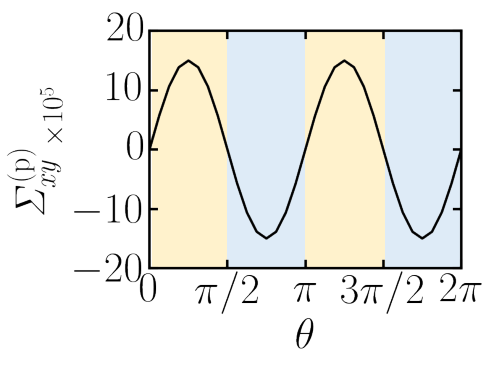
\includegraphics[scale=0.8]{/Users/taiga/Projects/lab/thesis/components/chapter3/figs/bottom_heavy_torque.pdf}
        \caption{単体squirmerの存在による応力の$xy$成分}
        \label{fig:stresslet_xy}
    \end{figure}

\noindent
このグラフより,粒子の進行方向がオレンジ色で示した範囲内に固定される場合には,系の応力を大きくする方向に働き,
水色で示した範囲内に固定される場合には,系の応力を小さくする方向に働くことが分かる.
一方,粒子が定常的に回転している場合には,粒子の存在による応力の時間平均をとると,プラスとマイナスで打ち消し合い,系に影響は与えないと予想される.
